\subsubsection{Solar Thermal}
The calculation of the potential of solar thermal modules was done as described in Struckmann (2008) \citen{struckmann2008}. According to Struckmann (2008) the useful energy gain $Q_U$ of a solar thermal module is calculated with the formula shown in Equation \ref{eq:st_calc}. Figure \ref{fig:st_module} shows a sketch of a typical solar thermal module and shows the parameter, which are necessary to compute $Q_U$  

\begin{align}
\label{eq:st_calc}
Q_U &= F_R  A \left( I \tau \alpha - U_L \left(T_i - T_a \right) \right)\\\notag\\\notag
\text{with:}&\\\notag
F_R &:\text{ Efficiency Coefficient of the module}\\\notag
A &: \text{ module area, $m^2$}\\\notag
I &: \text{ Solar radiation, $W/m^2$ }\\\notag
\tau &: \text{ transmission coefficient of glazing}\\\notag
\alpha &: \text{ absorption coefficient of plate}\\\notag
U_L &: \text{ collector overall heat loss coefficient, $W/m^2$}\\\notag
T_i &: \text{ input fluid temperature, $^\circ C$}\\\notag
T_a &: \text{ average outside air temperature, $^\circ C$}\notag
\end{align}

\begin{figure}[ht]
	\centering
	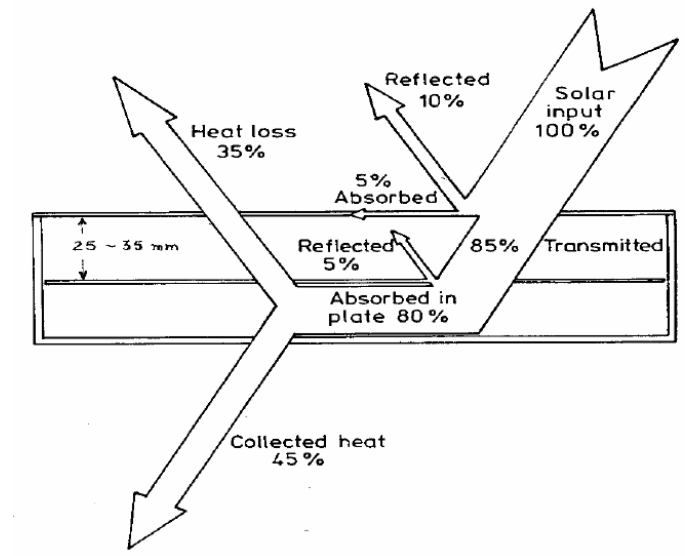
\includegraphics[width=0.5\textwidth]{phase2/group2/figure/st_module.png}
	\caption{typical module with visualization of calculation parameters (Struckmann (2008))}
	\label{fig:st_module}
\end{figure}

For the calculation of the potential a standard solar thermal module has been taken, the TitanPower-AL2DH Flat Plate Collector from the company SunMaxxSolar \citen{sunmaxx}. The efficiency coefficient is assumed to be $F_R = 0.35$ since this value is also used by SimuPLAN for Solar Atlas Berlin. The input fluid temperature is assumed to be $T_i = 10 ^\circ C$ which seems to be a realistic value for the region of Berlin.  Also the average outside air temperature is taken as  $T_a = 10 ^\circ C$.

